\label{nagrywanie_obrazu} Po zakończeniu pobierania obrazu instalatora należy nagrać go na zewnętrzny nośnik i uruchomić komputer z tego nośnika. Najlepszym rozwiązaniem jest użycie klucza USB (pendrive'a), gdyż obrazy instalacyjne Ubuntu są zbyt duże, aby zmieściły się na typowych krążkach CD o pojemności 700 MB. Weź jednak pod uwagę, że nie wszystkie komputery potrafią startować z klucza USB. Jeżeli twój komputer nie pozwala na wykonanie takiej operacji, będziesz musiał użyć płyty DVD lub karty (micro)SD.

\subsubsection{System Windows 7/8, nagrywanie na płytę DVD}
%TODO zweryfikować, czy Windows 8 też to ma
\begin{wrapfigure}[10]{r}{0.5\textwidth}
	\vspace{-10pt}
	\begin{tikzpicture}
	\node[anchor=south west,inner sep=0] (image) at (0,0) {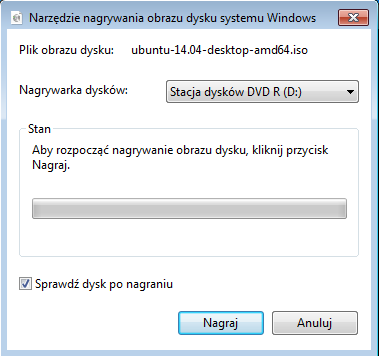
\includegraphics[width=\linewidth]{images/instalacja_nagrywanie_obrazu_DVD.png}};
	\begin{scope}[x={(image.south east)},y={(image.north west)}]
		\draw[ubuntu_orange,line width=3pt,rounded corners] (0.42,0.70) rectangle (0.96,0.79);
		\draw[ubuntu_orange,line width=3pt,fill=white,fill opacity=0.75] (0.35,0.75) circle [radius=0.30cm]
			node[text=black]{\Large \textbf 1};
		\draw[ubuntu_orange,dashed,line width=3pt] (0.40,0.75) -- (0.42,0.75);
		
		\draw[ubuntu_orange,line width=3pt,rounded corners] (0.02,0.16) rectangle (0.48,0.24);
		\draw[ubuntu_orange,line width=3pt,fill=white,fill opacity=0.75] (0.55,0.35) circle [radius=0.30cm]
			node[text=black]{\Large \textbf 3};
		\draw[ubuntu_orange,dashed,line width=3pt] (0.51,0.35) -- (0.22,0.23);
		
		\draw[ubuntu_orange,line width=3pt,rounded corners] (0.46,0.05) rectangle (0.71,0.15);
		\draw[ubuntu_orange,line width=3pt,fill=white,fill opacity=0.75] (0.85,0.25) circle [radius=0.30cm]
			node[text=black]{\Large \textbf 4};
		\draw[ubuntu_orange,dashed,line width=3pt] (0.81,0.25) -- (0.65,0.15);

    \end{scope}
\end{tikzpicture}
\end{wrapfigure}

Systemy operacyjne Windows 7 i 8 mają wbudowane narzędzie do wypalania plików .iso na płytach. Kliknij prawym przyciskiem myszy na pobrany obraz instalatora Ubuntu i wybierz opcję \textcolor{ubuntu_orange}{Nagraj obraz dysku}, a następnie:

\begin{enumerate}[label=\protect\circled{\arabic*}]
\item z tej listy wybierz swoją nagrywarkę;
\item włóż do wybranego napędu czystą płytę DVD;
\item upewnij się, że zaznaczone jest pole \textcolor{ubuntu_orange}{Sprawdź dysk po nagraniu};
\item kliknij przycisk \textcolor{ubuntu_orange}{Nagraj}.
\end{enumerate}
\vspace{1cm}
\subsubsection{System Windows XP i inne wersje, nagrywanie na płytę DVD}
\begin{wrapfigure}[11]{r}{0.5\linewidth}
	\vspace{-10pt}
	\begin{tikzpicture}
	\node[anchor=south west,inner sep=0] (image) at (0,0) {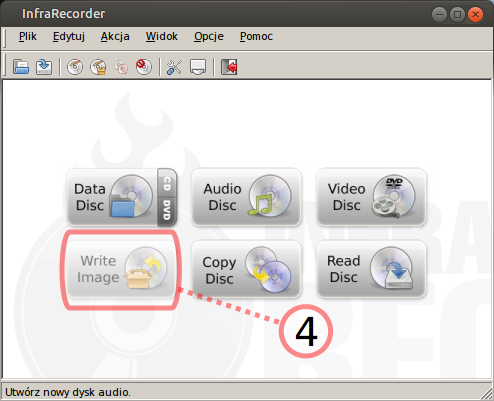
\includegraphics[width=\linewidth]{images/instalacja_nagrywanie_obrazu_DVD_winXP.png}};
	\begin{scope}[x={(image.south east)},y={(image.north west)}]
		\draw[ubuntu_orange,line width=3pt,rounded corners] (0.13,0.24) rectangle (0.37,0.42);
		\draw[ubuntu_orange,line width=3pt,fill=white,fill opacity=0.75] (0.55,0.15) circle [radius=0.30cm]
			node[text=black]{\Large \textbf 4};
		\draw[ubuntu_orange,dashed,line width=3pt] (0.51,0.15) -- (0.37,0.35);

    \end{scope}
\end{tikzpicture}
\end{wrapfigure}

Starsze wersje systemu Windows nie mają wbudowanej możliwości nagrywania płyt DVD. Potrzebne będzie do tego osobne narzędzie. Obsługa tych programów jest bardzo podobna: należy wybrać opcję \textcolor{ubuntu_orange}{Nagrywanie obrazu na płytę}. Koniecznie nagrywaj z~wykorzystaniem tej opcji, gdyż inne (np. ,,Nagrywanie płyty z~danymi'' lub ,,Tworzenie kopii zapasowej'') utworzą dysk, którego nie będzie można użyć do uruchomienia komputera. Dla przykładu posłużymy się programem Infra Recorder.

\begin{enumerate}[label=\protect\circled{\arabic*}]
\item Pobierz i zainstaluj program \href{http://infrarecorder.org/?page_id=5}{Infra Recorder}.
\item Uruchom zainstalowany przed momentem program.
\item Włóż czystą płytę DVD do nagrywarki.
\item W programie Infra Recorder wybierz opcję \textcolor{ubuntu_orange}{Write Image}.
\item Wybierz pobrany wcześniej obraz instalatora systemu Ubuntu.
\item Kliknij przycisk \textcolor{ubuntu_orange}{OK}.
\end{enumerate}
\clearpage
\subsubsection{System Windows (każda wersja), nagrywanie na pendrive}
\begin{wrapfigure}[6]{r}{0.5\textwidth}
	\vspace{-10pt}
		
	\begin{tikzpicture}
	\node[anchor=south west,inner sep=0] (image) at (0,0) {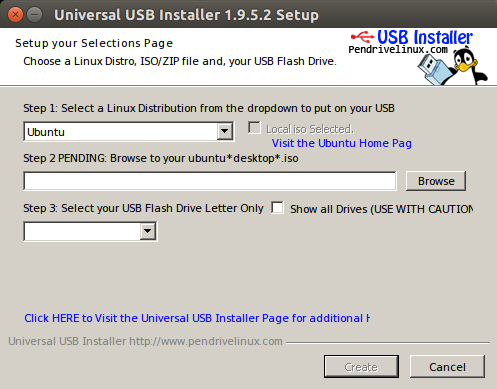
\includegraphics[width=\linewidth]{images/instalacja_nagrywanie_obrazu.png}};
	\begin{scope}[x={(image.south east)},y={(image.north west)}]
		\draw[ubuntu_orange,line width=3pt,rounded corners] (0.03,0.62) rectangle (0.50,0.70);
		\draw[ubuntu_orange,line width=3pt,fill=white,fill opacity=0.75] (0.95,0.65) circle [radius=0.30cm]
			node[text=black]{\Large \textbf 5};
		\draw[ubuntu_orange,dashed,line width=3pt] (0.91,0.65) -- (0.50,0.65);
		
		\draw[ubuntu_orange,line width=3pt,rounded corners] (0.03,0.50) rectangle (0.82,0.57);
		\draw[ubuntu_orange,line width=3pt,fill=white,fill opacity=0.75] (0.95,0.525) circle [radius=0.30cm]
			node[text=black]{\Large \textbf 6};
		\draw[ubuntu_orange,dashed,line width=3pt] (0.91,0.525) -- (0.82,0.525);
		
		\draw[ubuntu_orange,line width=3pt,rounded corners] (0.03,0.37) rectangle (0.33,0.44);
		\draw[ubuntu_orange,line width=3pt,fill=white,fill opacity=0.75] (0.95,0.40) circle [radius=0.30cm]
			node[text=black]{\Large \textbf 7};
		\draw[ubuntu_orange,dashed,line width=3pt] (0.91,0.4) -- (0.32,0.40);
		
		\draw[ubuntu_orange,line width=3pt,rounded corners] (0.64,0.02) rectangle (0.81,0.10);
		\draw[ubuntu_orange,line width=3pt,fill=white,fill opacity=0.75] (0.45,0.05) circle [radius=0.30cm]
			node[text=black]{\Large \textbf 8};
		\draw[ubuntu_orange,dashed,line width=3pt] (0.48,0.05) -- (0.64,0.05);
    \end{scope}
\end{tikzpicture}
\end{wrapfigure}

Jeżeli chcesz użyć pendrive'a jako nośnika instalacyjnego, upewnij się, że ma on przynajmniej 1 GB pojemności (w przeciwnym wypadku instalator się tam po prostu nie zmieści). Jeżeli masz już przygotowany pendrive, wykonaj po kolei następujące kroki:

\begin{enumerate}[label=\protect\circled{\arabic*}]
\item pobierz program \href{http://www.pendrivelinux.com/downloads/Universal-USB-Installer/Universal-USB-Installer-1.9.5.2.exe}{Universal USB Installer};
\item podłącz pendrive do komputera;
\item uruchom pobrany program;
\item zaakceptuj umowę licencyjną;
\item z tej listy wybierz Ubuntu;
\item kliknij przycisk \textcolor{ubuntu_orange}{Browse} i wskaż pobrany wcześniej obraz instalatora Ubuntu;
\item z tej listy wybierz podłączony wcześniej pendrive;\\
\textbf{UWAGA: Wszystkie dane na nim zostaną skasowane!}
\item kliknij przycisk \textcolor{ubuntu_orange}{Create};
\item Poczekaj na zakończenie operacji.
\end{enumerate}

\subsubsection{System Linux, nagrywanie na pendrive}
\begin{wrapfigure}{r}{0.5\textwidth}
	\vspace{-10pt}
	\begin{tikzpicture}
	\node[anchor=south west,inner sep=0] (image) at (0,0) {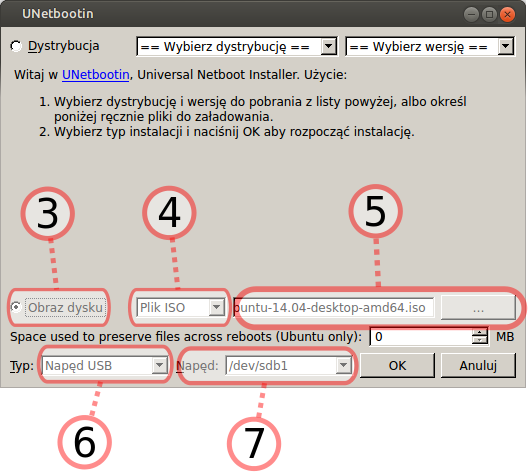
\includegraphics[width=\linewidth]{images/instalacja_nagrywanie_obrazu_linux.png}};
	\begin{scope}[x={(image.south east)},y={(image.north west)}]
		\draw[ubuntu_orange,line width=3pt,rounded corners] (0.01,0.18) rectangle (0.21,0.23);
		\draw[ubuntu_orange,line width=3pt,fill=white,fill opacity=0.75] (0.10,0.45) circle [radius=0.30cm]
			node[text=black]{\Large \textbf 3};
		\draw[ubuntu_orange,dashed,line width=3pt] (0.10,0.40) -- (0.10,0.22);
		
		\draw[ubuntu_orange,line width=3pt,rounded corners] (0.22,0.18) rectangle (0.43,0.23);
		\draw[ubuntu_orange,line width=3pt,fill=white,fill opacity=0.75] (0.33,0.45) circle [radius=0.30cm]
			node[text=black]{\Large \textbf 4};
		\draw[ubuntu_orange,dashed,line width=3pt] (0.33,0.40) -- (0.33,0.22);
		
		\draw[ubuntu_orange,line width=3pt,rounded corners] (0.43,0.18) rectangle (0.99,0.23);
		\draw[ubuntu_orange,line width=3pt,fill=white,fill opacity=0.75] (0.70,0.45) circle [radius=0.30cm]
			node[text=black]{\Large \textbf 5};
		\draw[ubuntu_orange,dashed,line width=3pt] (0.70,0.40) -- (0.70,0.22);
		
		\draw[ubuntu_orange,line width=3pt,rounded corners] (0.07,0.02) rectangle (0.32,0.10);
		\draw[ubuntu_orange,line width=3pt,fill=white,fill opacity=0.75] (0.04,0.06) circle [radius=0.30cm]
			node[text=black]{\Large \textbf 6};
		
		\draw[ubuntu_orange,line width=3pt,rounded corners] (0.43,0.02) rectangle (0.67,0.10);
		\draw[ubuntu_orange,line width=3pt,fill=white,fill opacity=0.75] (0.40,0.06) circle [radius=0.30cm]
			node[text=black]{\Large \textbf 7};

	\end{scope}
\end{tikzpicture}
\end{wrapfigure}

W systemach operacyjnych Linux do nagrywania obrazu na pendrive najlepiej posłużyć się programem \textcolor{ubuntu_orange}{UNetbootin}, dostępnym w większości popularnych dystrybucji. UNetbootin rozpakuje pobrany obraz instalatora (plik .iso) bezpośrednio na pendrive, a następnie zainstaluje na nim program rozruchowy.

Sposób uruchomienia instalatora (opisywany w dalszej części tego przewodnika) nieco się różni, jeżeli użyłes programu UNetbootin. Po uruchomieniu komputera z tak przygotowanego pendrive'a wyświetlony zostanie niebieski ekran z opcjami instalacji, ale bez możliwości wyboru języka. Nazwy opcji są identyczne z tymi opisanymi w rozdziale \ref{instalacja_uruchomienie_uefi}: Uruchomienie instalatora UEFI. Różnią się one tylko szatą graficzną.
\begin{enumerate}[label=\protect\circled{\arabic*}]
\item Zainstaluj UNetBootIn korzystając ze swojego menadżera pakietów.
\item Uruchom zainstalowany przed momentem program.
\item Zaznacz pole ,,Obraz dysku''.
\item Z menu wybierz ,,Plik ISO''.
\item W tym polu podaj ścieżkę do pobranego wcześniej obrazu instalatora Ubuntu. Wciśnij przycisk oznaczony trzema kropkami (,,\ldots'') i wskaż plik.
\item W tym menu wybierz Napęd USB.
\item Z tego menu wybierz podłączony wcześniej pendrive.\\
\textbf{UWAGA: Wszystkie dane znajdujące się na tym nośniku zostaną skasowane!}
\item Kliknij przycisk \textcolor{ubuntu_orange}{OK}, aby rozpocząć nagrywanie.
\end{enumerate}

\subsubsection{System Linux, nagrywanie na DVD}
\begin{wrapfigure}[10]{r}{0.5\linewidth}
	\vspace{-10pt}
	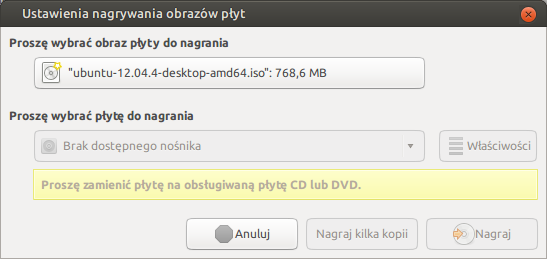
\includegraphics[width=\linewidth]{images/instalacja_nagrywanie_obrazu_linux_DVD.png}
\end{wrapfigure}

Aby nagrać obraz na płytę DVD, potrzebujesz odpowiedniego programu. W tym przykładzie posłużymy się dostępną w większości dystrybucji nagrywarką Brasero. Kliknij prawym przyciskiem myszy na pobrany wcześniej obraz instalatora Ubuntu i wybierz
\menu{{Otwórz w \ldots}>{Brasero}}. W otwartym oknie zostaniesz poproszony o włożenie czystej płyty DVD. Zrób to, a następnie kliknij przycisk \textcolor{ubuntu_orange}{Nagraj}.
